%%%%%%%%%%%%%%%%%%%%%%%%%%%%%%%%%%%%%%%%%%%%%%%%%%%%%%%%%%%%%%%%%%%%%%
%%                     module
%%%%%%%%%%%%%%%%%%%%%%%%%%%%%%%%%%%%%%%%%%%%%%%%%%%%%%%%%%%%%%%%%%%%%%
\color{green}
\subsection{\glyph{Submap}}\label{sec:submap}

A \glyph{submap} is used to encapsulate a certain number of processes (including all types of nodes and edges) within one glyph. The module hides its content to the users, and display only input terminals (or ports). A module is not equivalent to an omitted process (see section~\ref{sec:omitted}). In the case of an SBGN map available through a software tool, the content of a module may be available to the tool. A user could then ask the tool to expand the module, for instance by clicking on the module icon, that would expand the module within the same map (on the same canvas) or open it in a different canvas.

\begin{description}
\item[SBO term:]\mbox{}\\ to be determined
\item[container:]\mbox{}\\ The \glyph{submap} is represented as a square box, to remind that it is fundamentaly a process.
\item[label:] \mbox{}\\ The identification of the \glyph{submap} is carried by an unbordered box containing a string of
  characters. The characters may be distributed on several lines to improve readability, although this is not mandatory.  The label box has to be attached to the center of the container box.
\item[auxiliary items:]\mbox{}\\ A \glyph{submap} carries labeled terminals. When the submap is represented folded, those terminals are linked to external EPNs (section~\ref{sec:EPNs}) or containers (section~\ref{sec:CNs}). In the unfolded view, exposing the internal structure of the submap, a set of \glyph{tags} point to the corresponding internal EPNs (section~\ref{sec:EPNs}) or containers (section~\ref{sec:CNs}).
\end{description}

\begin{center}
\scalebox{0.5}{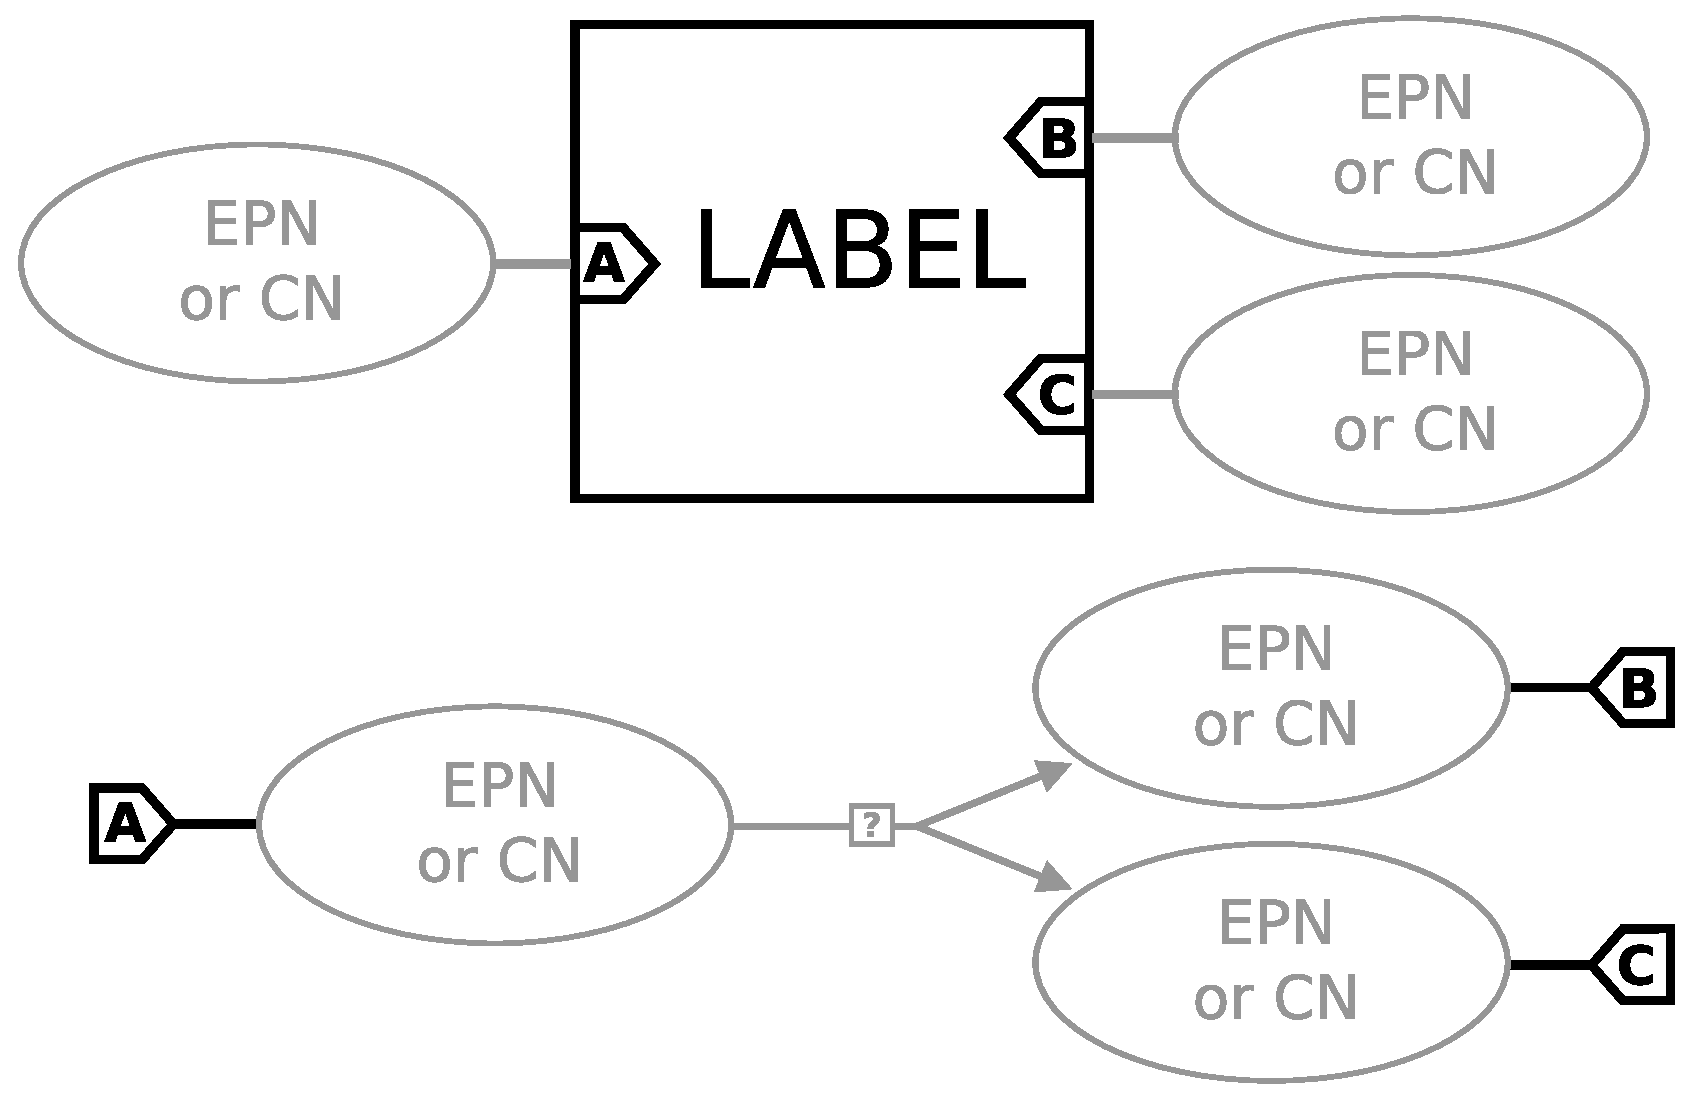
\includegraphics{images/submap.eps}}
\end{center}

The following map represents a \glyph{submap} that transforms glucose into fructose-6-phosphate. The \glyph{submap} carry five terminals, four linked to EPNs and one linked to a \glyph{compartment}. The latter is particularly important in the case of EPNs present only in a \glyph{compartment} enclosed in a \glyph{submap}, and that are not linked to terminals themselves. Note that the terminals do not define a ``direction'', such as input or output. The flux of the reactions is determined by the context.

\begin{center}
\scalebox{0.5}{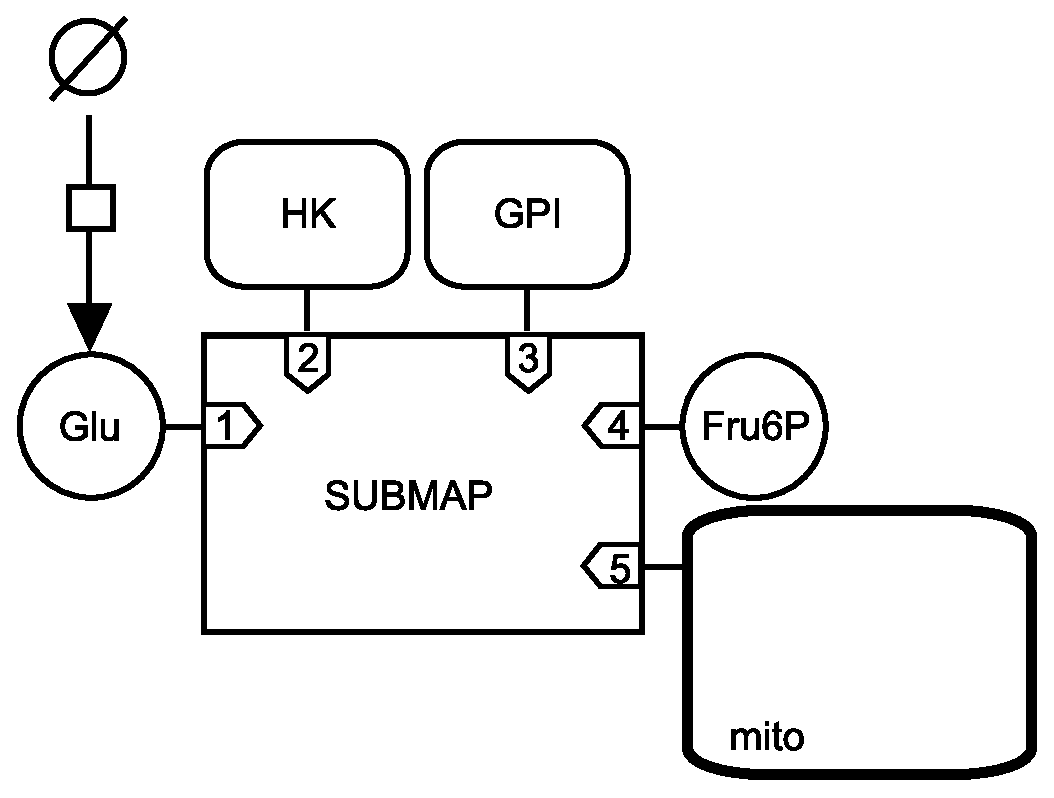
\includegraphics{examples/submap-folded.eps}}
\end{center}

The following map represents the unfolded version of the above, displaying the reactions enclosed in the module \emph{in the same canvas}. Note the terminal 5, linking the compartment ``mitom'' of the submap to the to the compartment ``mito'' outside the submap. The compartment containing Glu6P is implicitely defined as the same than the compartment containing Glum and Fru6pm. There is no ambiguity because if Glu and Fru6m were in different compartments, one of them should have been defined within the submap.

\begin{center}
\scalebox{0.5}{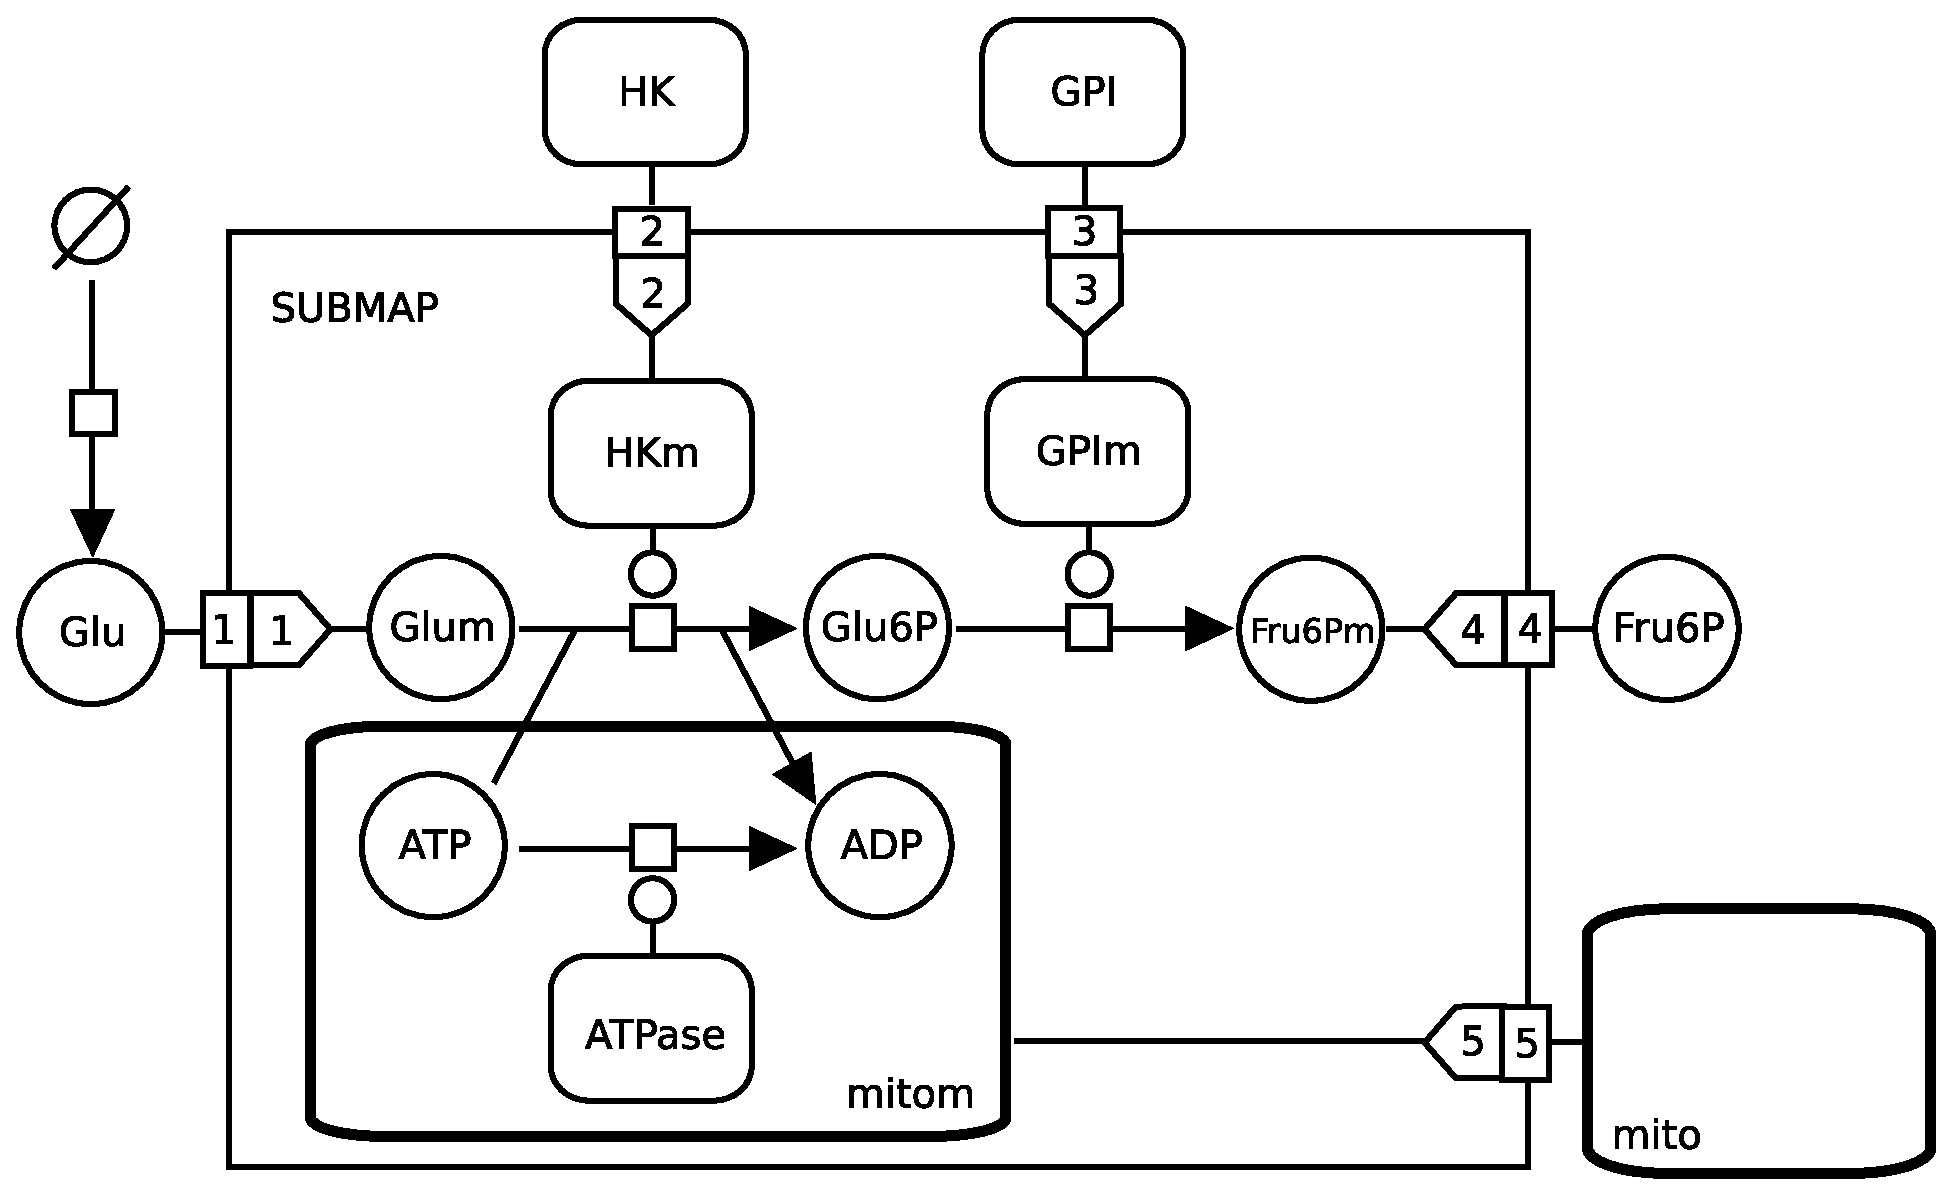
\includegraphics{examples/submap-unfolded.eps}}
\end{center}

The following map represents another unfolded version of the above, displaying the reactions enclosed in the submap \emph{in a different canvas}. Here, the anything outside the submap has disappeared, and the internal \glyph{tags} are not linked to the corresponding external \glyph{units of information}.

\begin{center}
\scalebox{0.5}{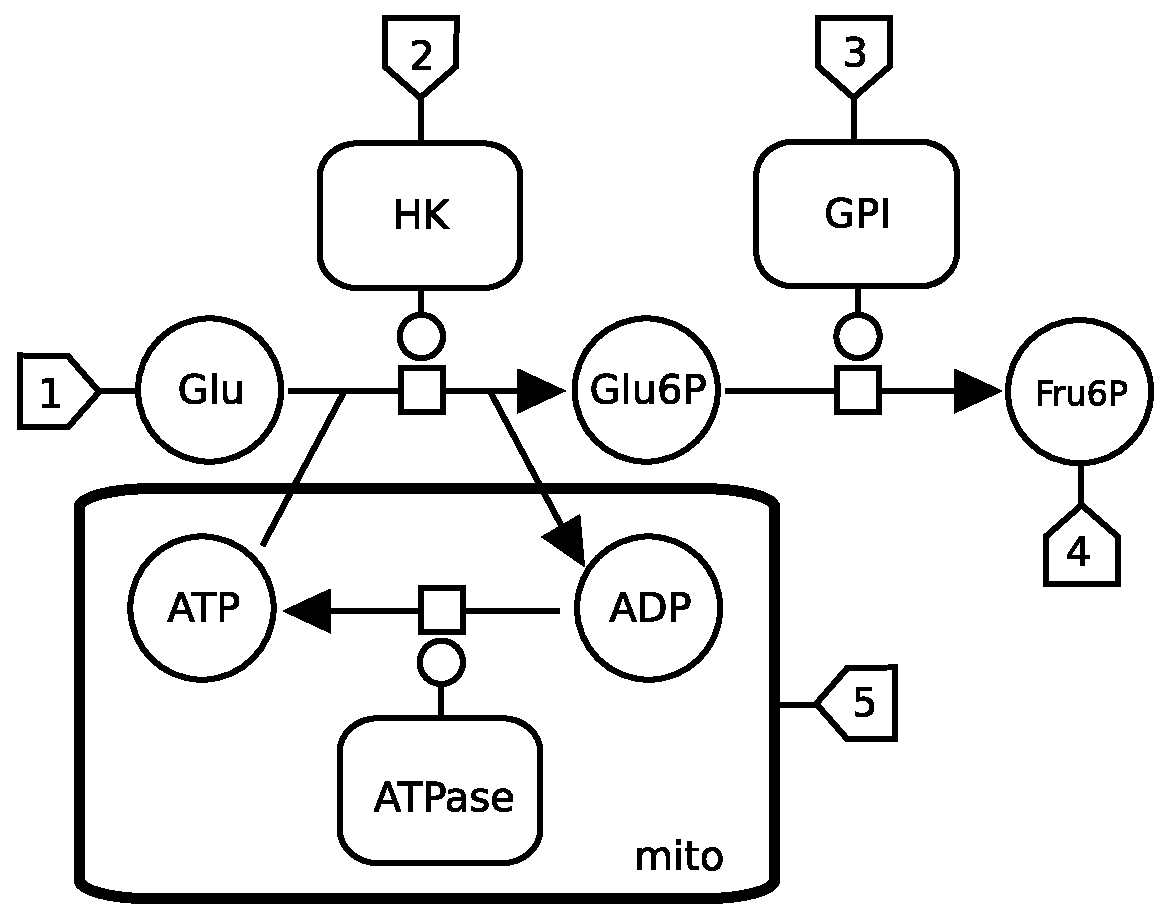
\includegraphics{examples/submap-dissociated.eps}}
\end{center}
\normalcolor

